\section{Detailed system architecture}

\begin{figure}[!ht]
    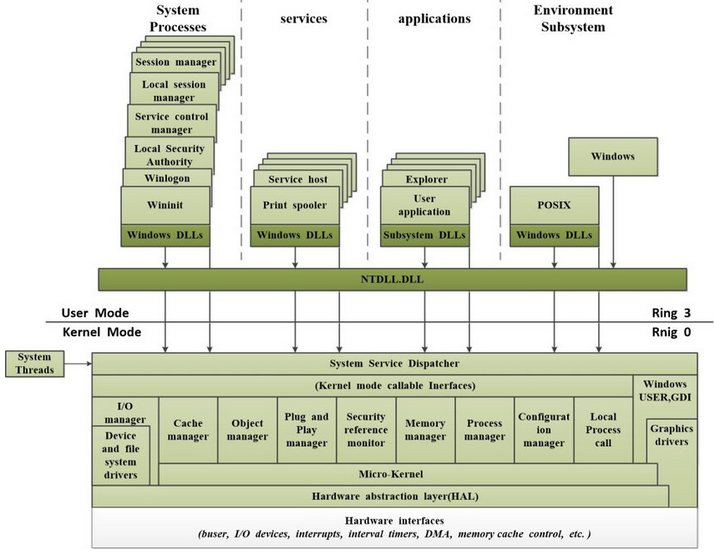
\includegraphics[width=\linewidth]{knowledge/internals/images/detailed-archi.png}
    \caption{Detailed archi}
    \label{fig:windows_detailed_archi}
\end{figure}


\subsection{Environment subsystems and subsystem DLLs}

\subsubsection{Introduction}
\begin{itemize}
    \item {\bf Environment subsystem} expose some subset of the base Windows executive system services to application programs. 
    \item Each subsystem can provide access to different subsets of the native services in Windows.
    \item Each executable image is bound to one and only one subsystem.
    \item When an image is run, the process creation code examines the subsystem type code in the image header so that it can notify the proper subsystem of the new process
    \item user applications don’t call Windows system services directly. Instead, they go through one or more subsystem DLLs.
    \item The {\bf environment subsystem processes}, running in user mode, are responsible for maintaining the state of the client applications running under their control.
\end{itemize}

When an application calls a function in a subsystem DLL, one of three things can occur:
\begin{itemize}
    \item The function is entirely implemented in user mode inside the subsystem DLL.
    \item The function requires one or more calls to the Windows executive.
    \item The function requires some work to be done in the environment subsystem process. In this case, a client/server request is made to the environment subsystem via an ALPC message sent to the subsystem to perform some operation. The subsystem DLL then waits for a reply before returning to the caller.
\end{itemize}

Some functions can be a combination of the second and third items just listed.

\subsubsection{Subsystem startup}
Subsystems are started by the Session Manager subsystem (SMSS) according to \verb+HKLM\SYSTEM\CurrentControlSet\Control\Session Manager\SubSystems+ 
\begin{itemize}
    \item \verb+Required+ value: list String that must be defined as registry value and define the list of the subsystems that load when the system boots
    \item \verb+Optional+ value: (load on demand) 
    \item \verb+kmode+: contains the file name of the kernel-mode portion of the Windows subsystem, \verb+Win32k.sys+
\end{itemize}

\subsubsection{Windows subsystem}

{\bf All subsystem rely on Windows subsystem to perform display I/O.}

The Windows subsystem consists of the following major components:
\begin{itemize}
    \item For each session, an instance of the \href{https://medium.com/@ijaz.faheem/windows-environment-subsystems-csrss-synch-with-windows-kernel-on-the-windows-user-process-164d57f2a81b}{CSRSS} loads four DLLs (\verb+Basesrv.dll+, \verb+Winsrv.dll+, \verb+Sxssrv.dll+, and \verb+Csrsrv.dll+) that contain support for the following:
        \begin{itemize}
            \item Various housekeeping tasks related to creating and deleting processes and threads
            \item Shutting down Windows applications
            \item Sending certain kernel notification messages to Windows applications as Window messages
            \item Side-by-Side (SxS)/Fusion and manifest cache support
            \item Several natural language support functions, to provide caching
        \end{itemize}
    \item A {\bf kernel-mode device driver} (Win32k.sys) that contains the following:
        \begin{itemize}
            \item The window manager (controls window displays; manages screen output; collects input
            from keyboard, mouse, and other devices; and passes user messages to applications)
            \item The Graphics Device Interface (GDI), which is a library of functions for graphics output devices
            \item Wrappers for DirectX
        \end{itemize}
    \item The {\bf console host process} (Conhost.exe), which provides support for console (character cell)
    applications
    \item The Desktop Window Manager
    \item Subsystem DLLs
    \item Graphics device drivers
\end{itemize}

{\bf CSRSS}:

Windows Kernel creates the process and thread and returns the handles to the method CreateProcessInternal (Kernelbase.dll). The CreateProcessInternal performs security operations (e.g., SxS) and constructs and sends a message to the Csrss process. The message contains information about process \& thread handles, section objects, flags, and other required information etc.

The Csrss is a critical system process, and it is responsible for managing the graphical user interface (GUI) on Windows systems. It also creates the process and keeps them in the organized process list. The process also monitors the user mode processes, and it can terminate a process if it crashes or because of any security issue.

The Csrss takes the process and thread handles and creates the duplicate process(\verb+CSR_Process+) and thread(\verb+CSR_Thread+) to monitor the process for Windows Subsystem.

The Csrss push the new process into the windows-subsystem wide process list(aka managed processes) on the successful creation of the Csrss process.


{\bf Win32k.sys}

The basic window-management requirements for Windows 10–based devices vary considerably depending on the device in question. For these reasons, the functionality of Win32K.sys has been split among  several kernel modules so that not all modules may be required on a specific system. This significantly reduces the attack surface of the window manager by reducing the complexity of the code and eliminating many of its legacy pieces.

Applications call the standard USER functions to create user-interface controls, such as windows and buttons, on the display. The window manager communicates these requests to the GDI, which passes them to the graphics device drivers, where they are formatted for the display device. A display driver is paired with a video miniport driver to complete video display support.

The GDI provides a set of standard two-dimensional functions that let applications communicate with graphics devices without knowing anything about the devices. GDI functions mediate between applications and graphics devices such as display drivers and printer drivers. The GDI interprets application requests for graphic output and sends the requests to graphics display drivers. It also provides a standard interface for applications to use varying graphics output devices. This interface enables application code to be independent of the hardware devices and their drivers. The GDI tailors its messages to the capabilities of the device, often dividing the request into manageable parts.

Because much of the subsystem—in particular, display I/O functionality—runs in kernel mode, only a few Windows functions result in sending a message to the Windows subsystem process: process and thread creation and termination and DOS device drive letter mapping (such as through subst.exe). In general, a running Windows application won’t cause many, if any, context switches to the Windows subsystem process, except as needed to draw the new mouse cursor position, handle keyboard input, and render the screen through CDD.

{\bf Console window host}

\verb+Conhost.exe+ process is spawned from the console-based process by the console driver (\verb+ConDrv.sys+) The process console-based process communicates with \verb+Conhost.exe+ using the console driver (\verb+ConDrv.sys+), by sending read, write, I/O control and other I/O request types.

Conhost.exe is designated as a server and the process using the console is the client.

\subsubsection{Other subsystem, Pico providers and WSL}


\subsection{Ntdll.dll}

\verb+Ntdll.dll+ is a special system support library primarily for the use of subsystem DLLs and images natives (not tied to a particular subsystem) applications.

It contains two types of functions:
\begin{itemize}
    \item {\bf System service dispatch stubs} to Windows executive system services. For each of these functions, \verb+Ntdll.dll+ contains an entry point with the same name. The code inside the function contains the architecture-specific instruction that causes a transition into kernel mode to invoke the {\bf system service dispatcher}. After verifying some parameters, this system service dispatcher calls the actual kernel-mode system service that contains the real code inside \verb+Ntoskrnl.exe+
    
    \item {\bf Internal support functions} used by subsystems, subsystem DLLs, and other native images such as:
        \begin{itemize}
            \item image loader (\verb+Ldr+ prefix), 
            \item heap manager, 
            \item Windows subsystem process communication functions (\verb+Csr+ prefix)
            \item general run-time library routines (\verb+Rtl+ prefix)
            \item support for user-mode debugging (\verb+DbgUi+ prefix)
            \item Event Tracing for Windows (\verb+Etw+ prefix)
            \item user-mode asynchronous procedure call (APC) dispatcher and exception dispatcher
            \item a small subset of the C Run-Time (CRT) routines, limited to those routines that are part of the string and standard libraries (\verb+memcpy+, \verb+strcpy+, \verb+sprintf+)
        \end{itemize} 

\end{itemize}

\subsection{Executive}

\subsubsection{Object manager}
The object manager responsible for creating, deleting, protecting, and tracking Windows executive objects and abstract data types that are used to represent OS resources such as processes, threads, and the various synchronization objects.



\subsection{system service dispatcher}

{\bf Part 2 chapter 8 page 91}

The kernel's trap handlers dispatch interrupts, exceptions and system service calls.

\subsection{Kernel}

\subsection{Hardware abstraction layer}
\subsection{Device drivers}
\subsection{System processes}